\documentclass[11pt,oneside]{article}
\usepackage[T1]{fontenc}
\usepackage[utf8]{inputenc}
% \usepackage{lmodern}
%\usepackage[adobe-utopia,uppercase=upright,greeklowercase=upright]{mathdesign}
\usepackage[adobe-utopia]{mathdesign}
%\usepackage{minionpro}
% \usepackage{pifont}
% \usepackage{amssymb}
\usepackage{amsmath}
\usepackage[francais]{babel}
% \usepackage[francais]{varioref}
\usepackage[dvips]{graphicx}

\usepackage{framed}
\usepackage[normalem]{ulem}
\usepackage{fancyhdr}
\usepackage{titlesec}
\usepackage{vmargin}
\usepackage{longtable}

\usepackage{ifthen}


%\usepackage{epsfig}
\usepackage{subfig}

\usepackage{multirow}
\usepackage{multicol} % Portions de texte en colonnes
\usepackage{flafter}%floatants après la référence



\usepackage{color}
\usepackage{colortbl}


\definecolor{gris25}{gray}{0.75}
\definecolor{bleu}{RGB}{18,33,98}
\definecolor{bleuf}{RGB}{42,94,171}
\definecolor{bleuc}{RGB}{231,239,247}
\definecolor{rougef}{RGB}{185,18,27}
\definecolor{rougec}{RGB}{255,230,231}
\definecolor{vertf}{RGB}{103,126,82}
\definecolor{vertc}{RGB}{220,255,191}

\newenvironment{rem}[1][\hsize]%
{%
    \def\FrameCommand
    {%
\rotatebox{90}{\textit{\textsf{Remarque}}} 
        {\color{bleuf}\vrule width 3pt}%
        \hspace{0pt}%must no space.
        \fboxsep=\FrameSep\colorbox{bleuc}%
    }%
    \MakeFramed{\hsize#1\advance\hsize-\width\FrameRestore}%
}%
{\endMakeFramed}%


\newenvironment{contexte}[1][\hsize]%
{%
    \def\FrameCommand
    {%
\rotatebox{90}{\textit{\textsf{Contexte}}} 
        {\color{bleuf}\vrule width 3pt}%
        \hspace{0pt}%must no space.
        \fboxsep=\FrameSep\colorbox{bleuc}%
    }%
    \MakeFramed{\hsize#1\advance\hsize-\width\FrameRestore}%
}%
{\endMakeFramed}%

\newenvironment{savoir}[1][\hsize]%
{%
    \def\FrameCommand
    {%
\rotatebox{90}{\textit{\textsf{Savoir}}} 
        {\color{bleuf}\vrule width 3pt}%
        \hspace{0pt}%must no space.
        \fboxsep=\FrameSep\colorbox{bleuc}%
    }%
    \MakeFramed{\hsize#1\advance\hsize-\width\FrameRestore}%
}%
{\endMakeFramed}%

\newenvironment{prob}[1][\hsize]%
{%
    \def\FrameCommand%
    {%
\rotatebox{90}{\textit{\textsf{ Problématique}}} 
        {\color{rougef}\vrule width 3pt}%
        \hspace{0pt}%must no space.
        \fboxsep=\FrameSep\colorbox{rougec}%
    }%
    \MakeFramed{\hsize#1\advance\hsize-\width\FrameRestore}%
}%
{\endMakeFramed}%

\newenvironment{obj}[1][\hsize]%
{%
    \def\FrameCommand%
    {%
\rotatebox{90}{\textit{\textsf{ $\;$}}} 
        {\color{rougef}\vrule width 3pt}%
        \hspace{0pt}%must no space.
        \fboxsep=\FrameSep\colorbox{rougec}%
    }%
    \MakeFramed{\hsize#1\advance\hsize-\width\FrameRestore}%
}%
{\endMakeFramed}%

\newenvironment{defi}[1][\hsize]%
{%
    \def\FrameCommand%
    {%
\rotatebox{90}{\textit{\textsf{Définition\\}}} 
        {\color{bleuf}\vrule width 3pt}%
        \hspace{0pt}%must no space.
        \fboxsep=\FrameSep\colorbox{bleuc}%
    }%
    \MakeFramed{\hsize#1\advance\hsize-\width\FrameRestore}%
}%
{\endMakeFramed}%


\newenvironment{hypo}[1][\hsize]%
{%
    \def\FrameCommand%
    {%
\rotatebox{90}{\textit{\textsf{Hypothèse\\}}} 
        {\color{bleuf}\vrule width 3pt}%
        \hspace{0pt}%must no space.
        \fboxsep=\FrameSep\colorbox{bleuc}%
    }%
    \MakeFramed{\hsize#1\advance\hsize-\width\FrameRestore}%
}%
{\endMakeFramed}%


\newenvironment{prop}[1][\hsize]%
{%
    \def\FrameCommand%
    {%
\rotatebox{90}{\textit{\textsf{Propriété\\}}} 
        {\color{bleuf}\vrule width 3pt}%
        \hspace{0pt}%must no space.
        \fboxsep=\FrameSep\colorbox{bleuc}%
    }%
    \MakeFramed{\hsize#1\advance\hsize-\width\FrameRestore}%
}%
{\endMakeFramed}%

\newenvironment{props}[1][\hsize]%
{%
    \def\FrameCommand%
    {%
\rotatebox{90}{\textit{\textsf{Propriétés\\}}} 
        {\color{bleuf}\vrule width 3pt}%
        \hspace{0pt}%must no space.
        \fboxsep=\FrameSep\colorbox{bleuc}%
    }%
    \MakeFramed{\hsize#1\advance\hsize-\width\FrameRestore}%
}%
{\endMakeFramed}%

\newenvironment{exemple}[1][\hsize]%
{%
    \def\FrameCommand%
    {%
\rotatebox{90}{\textit{\textsf{Exemple\\}}} 
        {\color{vertf}\vrule width 3pt}%
        \hspace{0pt}%must no space.
        \fboxsep=\FrameSep\colorbox{vertc}%
    }%
    \MakeFramed{\hsize#1\advance\hsize-\width\FrameRestore}%
}%
{\endMakeFramed}%

\newenvironment{resultat}[1][\hsize]%
{%
    \def\FrameCommand%
    {%
\rotatebox{90}{\textit{\textsf{Résultat\\}}} 
        {\color{rougef}\vrule width 3pt}%
        \hspace{0pt}%must no space.
        \fboxsep=\FrameSep\colorbox{rougec}%
    }%
    \MakeFramed{\hsize#1\advance\hsize-\width\FrameRestore}%
}%
{\endMakeFramed}%

\newenvironment{methode}[1][\hsize]%
{%
    \def\FrameCommand%
    {%
\rotatebox{90}{\textit{\textsf{Méthode\\}}} 
        {\color{rougef}\vrule width 3pt}%
        \hspace{0pt}%must no space.
        \fboxsep=\FrameSep\colorbox{rougec}%
    }%
    \MakeFramed{\hsize#1\advance\hsize-\width\FrameRestore}%
}%
{\endMakeFramed}%

\newenvironment{theo}[1][\hsize]%
{%
    \def\FrameCommand%
    {%
\rotatebox{90}{\textit{\textsf{Théorème\\}}} 
        {\color{rougef}\vrule width 3pt}%
        \hspace{0pt}%must no space.
        \fboxsep=\FrameSep\colorbox{rougec}%
    }%
    \MakeFramed{\hsize#1\advance\hsize-\width\FrameRestore}%
}%
{\endMakeFramed}%

\newenvironment{warn}[1][\hsize]%
{%
    \def\FrameCommand%
    {%
\rotatebox{90}{\textit{\textsf{Attention\\}}} 
        {\color{rougef}\vrule width 3pt}%
        \hspace{0pt}%must no space.
        \fboxsep=\FrameSep\colorbox{rougec}%
    }%
    \MakeFramed{\hsize#1\advance\hsize-\width\FrameRestore}%
}%
{\endMakeFramed}%

% \usepackage{pstricks}
%\usepackage{minitoc}
% \setcounter{minitocdepth}{4}

\setcounter{tocdepth}{2}

% \mtcselectlanguage{french} 

%\usepackage{draftcopy}% "Brouillon"
% \usepackage{floatflt}
\usepackage{psfrag}
%\usepackage{listings} % Permet d'insérer du code de programmation
\renewcommand{\baselinestretch}{1.2}

% Changer la numérotation des figures :
% ------------------------------------
% \makeatletter
% \renewcommand{\thefigure}{\ifnum \c@section>\z@ \thesection.\fi
%  \@arabic\c@figure}
% \@addtoreset{figure}{section}
% \makeatother
 


%%%%%%%%%%%%
% Définition des vecteurs %
%%%%%%%%%%%%
 \newcommand{\vect}[1]{\overrightarrow{#1}}

%%%%%%%%%%%%
% Définition des torseusr %
%%%%%%%%%%%%

 \newcommand{\torseur}[1]{%
\left\{{#1}\right\}
}

\newcommand{\torseurcin}[3]{%
\left\{\mathcal{#1} \left(#2/#3 \right) \right\}
}

\newcommand{\torseurstat}[3]{%
\left\{\mathcal{#1} \left(#2\rightarrow #3 \right) \right\}
}

 \newcommand{\torseurc}[8]{%
%\left\{#1 \right\}=
\left\{
{#1}
\right\}
 = 
\left\{%
\begin{array}{cc}%
{#2} & {#5}\\%
{#3} & {#6}\\%
{#4} & {#7}\\%
\end{array}%
\right\}_{#8}%
}

 \newcommand{\torseurcol}[7]{
\left\{%
\begin{array}{cc}%
{#1} & {#4}\\%
{#2} & {#5}\\%
{#3} & {#6}\\%
\end{array}%
\right\}_{#7}%
}

 \newcommand{\torseurl}[3]{%
%\left\{\mathcal{#1}\right\}_{#2}=%
\left\{%
\begin{array}{l}%
{#1} \\%
{#2} %
\end{array}%
\right\}_{#3}%
}

 \newcommand{\vectv}[3]{%
\vect{V\left( {#1} \in {#2}/{#3}\right)}
}


\newcommand{\vectf}[2]{%
\vect{R\left( {#1} \rightarrow {#2}\right)}
}

\newcommand{\vectm}[3]{%
\vect{\mathcal{M}\left( {#1}, {#2} \rightarrow {#3}\right)}
}


 \newcommand{\vectg}[3]{%
\vect{\Gamma \left( {#1} \in {#2}/{#3}\right)}
}

 \newcommand{\vecto}[2]{%
\vect{\Omega\left( {#1}/{#2}\right)}
}
% }$$\left\{\mathcal{#1} \right\}_{#2} =%
% \left\{%
% \begin{array}{c}%
%  #3 \\%
%  #4 %
% \end{array}%
% \right\}_{#5}}

%  ------------------------------------------
% | Modification du formatage des sections : | 
%  ------------------------------------------

% Grands titres :
% ---------------

\newcommand{\titre}[1]{%
\begin{center}
      \bigskip
      \rule{\textwidth}{1pt}
      \par\vspace{0.1cm}
      
      \textbf{\large #1}
      \par\rule{\textwidth}{1pt}
    \end{center}
    \bigskip
  }

% Supprime le numéro du chapitre dans la numérotation des sections:
% -----------------------------------------------------------------
\makeatletter
\renewcommand{\thesection}{\@arabic\c@section}
\makeatother


% \titleformat{\chapter}[display]
% {\normalfont\Large\filcenter}
% {}
% {1pc}
% {\titlerule[1pt]
%   \vspace{1pc}%
%   \Huge}[\vspace{1ex}%
% \titlerule]


%%%% Chapitres Comme PY Pechard %%%%%%%%%
% numéro du chapitre
\DeclareFixedFont{\chapnumfont}{OT1}{phv}{b}{n}{80pt}
% pour le mot « Chapitre »
\DeclareFixedFont{\chapchapfont}{OT1}{phv}{m}{it}{40pt}
% pour le titre
\DeclareFixedFont{\chaptitfont}{T1}{phv}{b}{n}{25pt}

\definecolor{gris}{gray}{0.75}
\titleformat{\chapter}[display]%
	{\sffamily}%
	{\filleft\chapchapfont\color{gris}\chaptertitlename\
	\\
	\vspace{12pt}
	\chapnumfont\thechapter}%
	{16pt}%
	{\filleft\chaptitfont}%
	[\vspace{6pt}\titlerule\titlerule\titlerule]

%%%%  Fin Chapitres Comme PY Pechard %%%%%%%%%


% Section, subsection, subsubsection sans serifs :
% % ----------------------------------------------

% \makeatletter
% \renewcommand{\section}{\@startsection{section}{0}{0mm}%
% {\baselineskip}{.3\baselineskip}%
% {\normalfont\sffamily\Large\textbf}}%
% \makeatother

\makeatletter
\renewcommand{\@seccntformat}[1]{{\textcolor{bleu}{\csname
the#1\endcsname}\hspace{0.5em}}}
\makeatother

\makeatletter
\renewcommand{\section}{\@startsection{section}{1}{\z@}%
                       {-4ex \@plus -1ex \@minus -.4ex}%
                       {1ex \@plus.2ex }%
                       {\normalfont\Large\sffamily\bfseries}}%
\makeatother
 
\makeatletter
\renewcommand{\subsection}{\@startsection {subsection}{2}{\z@}
                          {-3ex \@plus -0.1ex \@minus -.4ex}%
                          {0.5ex \@plus.2ex }%
                          {\normalfont\large\sffamily\bfseries}}
\makeatother
 
\makeatletter
\renewcommand{\subsubsection}{\@startsection {subsubsection}{3}{\z@}
                          {-2ex \@plus -0.1ex \@minus -.2ex}%
                          {0.2ex \@plus.2ex }%
                          {\normalfont\large\sffamily\bfseries}}
\makeatother
 
\makeatletter             
\renewcommand{\paragraph}{\@startsection{paragraph}{4}{\z@}%
                                    {-2ex \@plus-.2ex \@minus .2ex}%
                                    {0.1ex}%               
{\normalfont\sffamily\bfseries}}
\makeatother
 
\makeatletter             
\renewcommand{\paragraph}{\@startsection{paragraph}{4}{\z@}%
                                    {-2ex \@plus-.2ex \@minus .2ex}%
                                    {0.1ex}%               
{\normalfont\sffamily\bfseries Question }}
\makeatother

\renewcommand{\theparagraph}{\arabic{paragraph}} 


\makeatletter
\renewcommand{\subparagraph}{\@startsection{subparagraph}{5}{\z@}%
                                       {-2ex \@plus-.1ex \@minus .2ex}%
                                       {0.1ex}%
				    {\normalfont\normalsize\sffamily\bfseries}}
\makeatletter
% \makeatletter
% \renewcommand{\subsection}{\@startsection{subsection}{1}{2mm}%
% {\baselineskip}{.3\baselineskip}%
% {\normalfont\sffamily\large\textbf}}%
% \makeatother
% 
% \makeatletter
% \renewcommand{\subsubsection}{\@startsection{subsubsection}{2}{4mm}%
% {\baselineskip}{.15\baselineskip}%
% {\normalfont\sffamily\large\textbf}}%
% \makeatother
% 
% \makeatletter
% \renewcommand{\paragraph}{\@startsection{paragraph}{3}{6mm}%
% {\baselineskip}{.15\baselineskip}%
% {\normalfont\sffamily\large\textbf}}%
% \makeatother
 
\setcounter{secnumdepth}{4}


%  --------
% | Marges |
%  --------


% \setmarginsrb{2.5cm}{1.5cm}{2.5cm}{2cm}{1cm}{1cm}{1cm}{1cm}
\setmarginsrb{1.5cm}{1cm}{1cm}{1.5cm}{1cm}{1cm}{1cm}{1cm}

% Changer les marges localement :
% -----------------------------
\newenvironment{changemargin}[2]{\begin{list}{}{%
\setlength{\topsep}{0pt}%
\setlength{\leftmargin}{0pt}%
\setlength{\rightmargin}{0pt}%
\setlength{\listparindent}{\parindent}%
\setlength{\itemindent}{\parindent}%
\setlength{\parsep}{0pt plus 1pt}%
\addtolength{\leftmargin}{#1}%
\addtolength{\rightmargin}{#2}%
}\item }{\end{list}}



\usepackage{pst-solides3d}
\usepackage{titletoc}
\titlecontents{chapter}[+3pc]
  {\addvspace{10pt}\sffamily\bfseries}
{\contentslabel[{\pscirclebox[fillstyle=solid,fillcolor=gray!25,
linecolor=gray!25,framesep=4pt]{\textcolor{white}{\thecontentslabel}}}]{2.5pc}}
  {}
  {\dotfill \normalfont\thecontentspage\ }

\titlecontents{section}[3pc]
  {\addvspace{2pt}\sffamily}
  {\contentslabel[\thecontentslabel]{1.8pc}}
  {}
  {\dotfill \normalfont\thecontentspage\ }

\titlecontents{subsection}[5pc]
  {\addvspace{2pt}\sffamily}
  {\contentslabel[\thecontentslabel]{1.8pc}}
  {}
  {\dotfill \normalfont\thecontentspage\ }

\titlecontents{subsubsection}[8pc]
  {\addvspace{2pt}\sffamily}
  {\contentslabel[\thecontentslabel]{3pc}}
  {}
  {\dotfill \normalfont\thecontentspage\ }
%{\;\titlerule\;\normalfont\thecontentspage\ }

\titlecontents{paragraph}[9pc]
  {\addvspace{2pt}\sffamily}
  {\contentslabel[\thecontentslabel]{3.5pc}}
  {}
  {\dotfill \normalfont\thecontentspage\ }




\usepackage[%
    pdftitle={Cinématique - DM5},
    pdfauthor={Xavier Pessoles},
    colorlinks=true,
    linkcolor=blue,
    citecolor=magenta]{hyperref}

\usepackage{schemabloc}

% \makeatletter \let\ps@plain\ps@empty \makeatother
%% DEBUT DU DOCUMENT
%% =================
\sloppy
\hyphenpenalty 10000

\newcommand{\Pointilles}[1][3]{%
\multido{}{#1}{\makebox[\linewidth]{\dotfill}\\[\parskip]
}}


\colorlet{shadecolor}{orange!15}

\newtheorem{theorem}{Theorem}

\newenvironment{theo}
  {\begin{snugshade}\begin{leftbar}\begin{theorem}}
  {\end{theorem}\end{leftbar}\end{snugshade}}


\renewenvironment{leftbar}[1][\hsize]
{%
    \def\FrameCommand
    {%
        {\color{bleuf}\vrule width 3pt}%
        \hspace{0pt}%must no space.
        \fboxsep=\FrameSep\colorbox{bleuc}%
    }%
    \MakeFramed{\hsize#1\advance\hsize-\width\FrameRestore}%
}
{\endMakeFramed}




\begin{document}


\newboolean{prof}
\setboolean{prof}{true}
%------------- En tetes et Pieds de Pages ------------
\pagestyle{fancy}
\renewcommand{\headrulewidth}{0pt}

\fancyhead{}
\fancyhead[L]{%
\begin{minipage}[c]{1.6cm}

\includegraphics[width=1.4cm]{png/logo_jh_ptsi.png}%
\end{minipage}
\rule{2cm}{.5pt}
}

\fancyhead[C]{\rule{12cm}{.5pt}}

\fancyhead[R]{%
\begin{minipage}[c]{3cm}
\begin{flushright}
\footnotesize{\textit{\textsf{Sciences Industrielles\\ pour l'Ingénieur}}}%
\end{flushright}
\end{minipage}
}

\renewcommand{\footrulewidth}{0.2pt}

\fancyfoot[C]{\footnotesize{\bfseries \thepage}}
\fancyfoot[L]{\footnotesize{2011 -- 2012} \\ X. \textsc{Pessoles}}
\ifthenelse{\boolean{prof}}{%
\fancyfoot[R]{\footnotesize{DM 5 -- CI 2 : SLCI -- P}}
}{%
\fancyfoot[R]{\footnotesize{DM 5 -- CI 2 : SLCI}}
}


%\begin{center}
%\textit{Centre d'intérêt}
%\end{center}

\begin{center}
 \Large\textsc{Devoir Maison 5}
\end{center}

\begin{center}
 \large\textsc{Éléments de corrigés} 
\end{center}

\vspace{.25cm}

\section{Mise en situation}
	
 
\section{Travail demandé}

\paragraph{}
\textit{Rechercher et expliquer ce que signifie le terme « pièces frettées ».}
Le frettage est un procédé d'assemblage de pièces, notamment pour des pièces cylindriques.
Dans ce procédé, l'arbre est plus grand que le moyeu. Afin d'assembler les deux pièces on chauffe le moyeu afin de le dilater ou on refroidit l'arbre afin de le contracter (ou les deux). La différence de température permet d'assembler les pièces. Une fois à même température, les pièces sont solidarisées.

%\paragraph{}
%\textit{Quel est le rôle de la pièce 38 ?}

\paragraph{}
\textit{Quels sont le nom et le rôle de la pièce 29 ?}

La pièce 29 est une goupille cannelée. Elle permet de réaliser une liaison encastrement entre deux pièces, ici les pièces 30 et 48. 

\paragraph{}
\textit{Quel est le rôle, dans le fonctionnement de ce mécanisme, du ressort 5 ?}

Le ressort 5 est un ressort de rappel. Lorsque le système n'est plus sous pression, le ressort permet de ramener le piston 10 vers la droite. 

\paragraph{}
\textit{Quel est le rôle du ressort 16 ?}

\paragraph{}
\textit{Rechercher ce que signifie précisément les désignations de matériaux donnés dans la nomenclature pour les pièces 5, 10, 38. Pour la pièce 10, vous expliciterez comment est déterminée la valeur 295. }

La pièce 5 est en $C\;60$. C'est un acier pour traitement thermique avec 0,06\% de carbone.

La pièce 10 est en $E\;295$. C'est un acier pour construction mécanique. La résistance élastique s'élève à $295 \; MPa$. Cette valeur est obtenue grâce à un essai de traction. 295 est la valeur maximale jusqu'à laquelle le matériau est élastique.

La pièce 38 est un  $Cu\; Sn \; 8 \; Pb\; 15$. C'est un alliage de cuivre. Il comporte 8\% d'étain et 15\% de plomb.


\paragraph{}
\textit{Donner l'ensemble des opérations qui ont mené à la fabrication des pièces 1, 3, 27 et 39. (En partant d'un lopin ou d'un lingot de métal, en arrivant à la forme finie.)}

La pièce 1 est composée de pans de tôle qui proviennent du laminage de l'acier. Ces pans sont alors soudés.

La pièce 3 semble avoir été moulée puis usinée (en fraisage).

La pièce 27 a probablement été forgée puis usinée (en perçage).

La pièce 39 semble avoir été laminée puis usinée (en tournage).

\subsection{Modélisation cinématique}
\paragraph{}
\textit{Déterminer les classes d'équivalence de ce mécanisme : pour ce faire, associer une couleur à chaque groupe défini, et « colorier » la vue de face en coupe A-A ainsi que les coupes B-B, C-C et D-D du plan d'ensemble. Faire également la liste des pièces par groupe et donner un nom a chaque groupe (utiliser le repère de la pièce principal du groupe).}

\begin{center}
\begin{tabular}{|c|c|c|}
\hline
Nom & Numéro & Pièces \\
\hline
\hline
Piston&		10&7,8,9,10,45,46,47\\
Tige&		28&28\\
Bras&			27&27,39,40,41\\
Balancier&		21&21, axe C\\
Bielle&		19&17,18,19,22\\
Crochet&		20&20\\
Galet	&	37&37,38\\
Bâti&			1&1,2,3,4,6,11,23,24,25,26,29,30,33,(42),43,48\\
Biellette&			15&12,13,14,15\\
\hline
\end{tabular}
\end{center}

\paragraph{}
\textit{Identifier les liaisons entre ces classes. Vous préciserez obligatoirement la nature des surfaces en contact, justifiant ainsi les liaisons déterminées. Donner le schéma plan et 3D des liaisons en respectant les couleurs choisies pour les classes d'équivalence de la question précédente. Le repère doit être identique pour tous les schémas.}
		
\begin{center}
\begin{tabular}{|c|c|p{.2\textwidth}|c|c|}
\hline
Groupes en liaison & Surfaces en contact & Liaison \\
\hline
\hline
10-1	&2 portions de cylindre& Pivot glissant d’axe $(A,\vect{x} )$ \\
\hline
10-28 &Cylindre + plan& Pivot d’axe $(B, \vect{z})$\\
\hline
28-27 &Cylindre + plan & Pivot d’axe $(C, \vect{z})$\\
\hline
27-21 & Cylindre + plan& Pivot d’axe $(C, \vect{z})$\\
\hline
27-1 &Cylindre + plan& Pivot d’axe $(D, \vect{z})$\\
\hline
21-37 &Cylindre + plan& Pivot d’axe $(F, \vect{z})$\\
\hline
37-20 &Cylindre et plan tangent& Linéaire rectiligne de normale $(J, \vect{v})$, de direction $\vect{z}$ \\
\hline
21-19 &Cylindre + plan& Pivot d’axe $(E, \vect{z})$\\
\hline
20-1 &Cylindre + plan& Pivot d’axe $(H,\vect{z} )$\\
\hline
20-15 &Cylindre + plan& Pivot d’axe $(G, \vect{z})$ \\
\hline
15-1&Cylindre&Linéaire annulaire d’axe $(I,  \vect{x})$\\
\hline
\end{tabular}
\end{center}


	
\paragraph{}
\textit{Effectuer le schéma cinématique plan de ce mécanisme, en couleurs (identiques aux classes d'équivalence) dans le plan de la coupe A-A, et à l'échelle du plan fourni.
 Utilisez  le plan pour positionner les centres et les axes des liaisons 
 Vous respecterez les solutions constructives choisies pour le mécanisme concernant les pièces qui seront considérées comme « axe » ou comme « alésage » de la liaison.}
\begin{center}
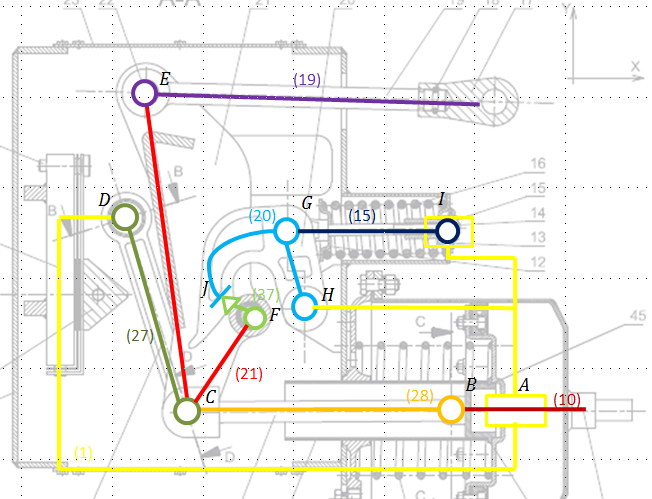
\includegraphics[width=.75\textwidth]{png/schema}
\end{center}

\paragraph{}
\textit{Effectuer un paramétrage pour chacun des types de liaisons. (Par exemple, s'il existe 3 pivots et 2 rotules dans le dessin, vous n'effectuerez qu'un seul paramétrage pour une des pivots et 1 paramétrage pour une des rotules.}


\paragraph{}
\textit{Effectuer ce schéma en perspective, en couleur.
 Son orientation est au choix.
 On ne demande pas de respecter l'échelle, mais vous devez respecter les positions relatives des liaisons}

\subsection{Étude technologique de certaines liaisons}

\subsection*{Analyse de la 1\iere solution}

\paragraph{}
\textit{Préciser la nature de la liaison entre la tige de piston 28 et le piston 10 dans la solution 1 présentée ci-dessous et décrire sa réalisation technologique.}

La liaison entre 28 et 10 est une liaison encastrement réalisée par soudage. 


\paragraph{}
\textit{A votre avis, quelle conséquence technique peut avoir le léger débattement angulaire de la tige 28 sur cette solution ? Justifier ainsi l'abandon de cette solution.}

Cette solution ne permet pas le débattement angulaire de la tige 28. Cette solution technologique risquerait de provoquer le coincement du piston dans la chambre.

\subsection*{Analyse de la 2\ieme solution}

\paragraph{}
\textit{Préciser la nature de la liaison entre la tige de piston 28 et le piston 10 dans cette solution 2.}

Cette liaison est une rotule.

\paragraph{}
\textit{Cette liaison résout-elle le problème du débattement angulaire mis en évidence dans la 1ere solution ? Justifier votre réponse.}

Cette liaison apporte du rotulage entre les deux pièces et évite ainsi le coincement du piston.


\paragraph{}
\textit{Quelle liaison a finalement été adoptée et quelle peut en être la raison ?}

Pour des raisons de coût et de facilité de réalisation il a été choisi d'utiliser une liaison pivot.

\subsection*{Analyse de la liaison 47/3}


\paragraph{}
\textit{En considérant qu'il n'y a aucun jeu possible,  quel modèle peut on proposer pour cette liaison.}

Dans ce cas, la liaison est modélisable par une liaison pivot glissant d'axe $(A,\vect{x})$.

\paragraph{}
\textit{Considérons maintenant qu'un léger jeu existe, impliquant un rotulage possible entre ces deux pièces, autour de deux axes supplémentaires. Quel modèle devrait-on alors adopter.}

Le rotulage ajoute 3 degrés de liberté en rotation à la liaison pivot glissant. La liaison est donc une linéaire annulaire (ou sphère cylindre) d'axe $(A,\vect{x})$.

\paragraph{}
\textit{L'usure observée au niveau de ce contact a tendance à augmenter ce jeu considérablement. Quelle solution simple pourriez vous proposer pour éviter cette usure.}
 
Pour éviter l'usure des pièces, on peut utiliser un coussinet.


\end{document}